%\mysubsection{Neutron-Neutron Angular Correlations in Fission}
The fission process is characterized by the emission of neutrons.
Neutron emission in fission can be classified into two categories depending on the time of emission: delayed and prompt.
Prompt fission neutrons are defined as neutrons that are emitted either immediately after ($<10^{-14}$ seconds) fission, or, during the scission of the nucleus, and account for $\sim99\%$ of neutron emission~\cite{Caldwell2017DelayedNs}.
Delayed neutrons are not relevant to the present work because they account for only $\sim1\%$ of total neutron emission in actinide photofission~\cite{Caldwell2017DelayedNs}, and, they are emitted milliseconds to minutes after fission, which is well outside the neutron acceptance timing window of the present work.

Prompt fission neutron production occurs by means of two distinct mechanisms.
The dominant mechanism is neutron emission from the fully accelerated fragments.
The second mechanism, referred to as \textit{early} or \textit{scission} neutron emission, is the emission of neutrons during either the scission of the nucleus or the acceleration of the fission fragments.
A large number of past studies have established that the majority of prompt fission neutrons (80\%--98\%) are emitted from the fully accelerated fragments, while scission neutrons account for the remaining 2\%--20\% percent~\cite{Scission2005}.
The nature of scission neutrons has remained elusive since their first tentative observation in 1962 by Bowman \emph{et al.}~\cite{Bowman}.

\mysubsection{Theoretical Basis}
%A useful observational input for prompt neutron modeling is the neutron-neutron (n-n) opening angle distribution of correlated neutron pairs, as seen in the lab frame, hereafter denoted $\theta_{nn}$.
The neutron-neutron (n-n) opening angle distribution of correlated neutron pairs, as seen in the lab frame, is widely used for the quantification of n-n angular correlations.
Angular correlations in fission neutrons arise due to the kinematics of the fission fragments.
%There are, on average, about 2 or 3 neutrons released per fission, depending on the target isotope and how the fission is induced.
It has been shown that neutrons released from the fully accelerated fission fragments are evaporated isotropically in the fragment's rest frame, and are emitted at speeds comparable to that of the fragments themselves~\cite{JORGENSEN}.
This leads to the well-known U--shaped distribution in neutron-neutron opening angle ($\theta_{nn}$), which has been reported in studies of neutron-induced, spontaneous, and, in this work, photofission.
An example of a typical $\theta_{nn}$ distribution is seen in Fig.~\ref{fig:Cf252_us_vs_them}.

The U--shaped distribution of $\theta_{nn}$ can be understood as the result of the boost provided to the neutrons by the fission fragments in binary fission.
Due to the conservation of momentum, the fully accelerated fission fragments are traveling nearly back-to-back, and neutrons emitted from different fragments are boosted in opposite directions, whereas neutrons emitted from the same fragment are boosted in the same direction.
Thus, because the velocities of the fission fragments are large enough to account for a significant portion of the kinetic energy of fission neutrons, neutron pairs emitted from the accelerated fragments exhibit a favoring of opening angles near 0$^{\circ}$ if emitted from the same fragment and 180$^{\circ}$ if emitted from different fragments, and, consequently, a suppression of opening angles near $90^{\circ}$.
% GAW - comment - is it kinetic energy or momentum? Sorry, long time since I thought about boosting between frames
% GAW - comment - Why is this even being mentioned here? I don't see yet how it fits in

The favoring of large and small n-n opening angles shows a strong dependence on neutron energy.
Neutrons with higher energy are more likely to have been emitted along the same direction as the fission fragments and are therefore expected to favor large and small opening angles.
The $\theta_{nn}$ distribution and its dependence on neutron energy are expected to shed light on several fundamental aspects of the fission process including the neutron multiplicity distributions associated with the light and heavy fission fragments, the nuclear temperatures of the fission fragments, and the mass distribution of the fission fragments as a function of energy released.
In addition, the unique kinematics of fission and the resulting n-n correlations have the potential to be the basis for a new tool to characterize fissionable materials~\cite{Talou2018}. % diifferential

%Furthermore, n-n opening angle measurements are useful for the study of scission neutrons.
%Scission neutrons are thought to be emitted isotropically in the lab frame, and so they have the effect of flattening out the U-shaped n-n opening angle distribution.
%Because of this effect, these measurements add to the growing breadth of nuclear data needed to confirm the exact extent of the scission-neutron component in fission, which remains an open problem in nuclear physics.


\mysubsection{Past Measurements: Spontaneous and Neutron Induced Fission}
%As of this writing, tabulated data for photofission is far scarcer than for neutron induced fission.
The first measurement of the angular correlation among coincident neutrons from fission was performed by Debenedetti \emph{et al.}~\cite{1948twoNCorr} in 1948 from neutron induced fission of $^{235}\text{U}$.
The next measurement of this type was performed by Pringle and Brooks in 1975~\cite{1975Cf252}, in which neutrons emitted from the spontaneous fission (SF) of $^{252}$Cf were found to have high coincidence rates at small opening angles near 0$^{\circ}$ and large opening angles near $180^{\circ}$.
In order to produce a result that is insensitive to the effects of detector geometry and efficiency, the present work uses techniques similar to those used in reference~\cite{1975Cf252}, in which a ratio is taken between a correlated opening angle distribution and an uncorrelated opening angle distribution.

To date, numerous measurements of n-n angular correlation using $^{252}$Cf have been performed~\cite{Verbeke2018, Pozzi2014, 2008CF252, 1975Cf252}.
This makes $^{252}$Cf a good benchmark for n-n angular correlation measurements.
Figure~\ref{fig:Cf252_us_vs_them} compares measurements in this work to past measurements of n-n correlations in the SF of $^{252}$Cf.
Correlated n-n measurements have also been performed using thermal induced fission of $^{235}$U, $^{233}$U, and $^{239}$Pu~\cite{Sokolov2010}.
\begin{figure}[h]
\centering
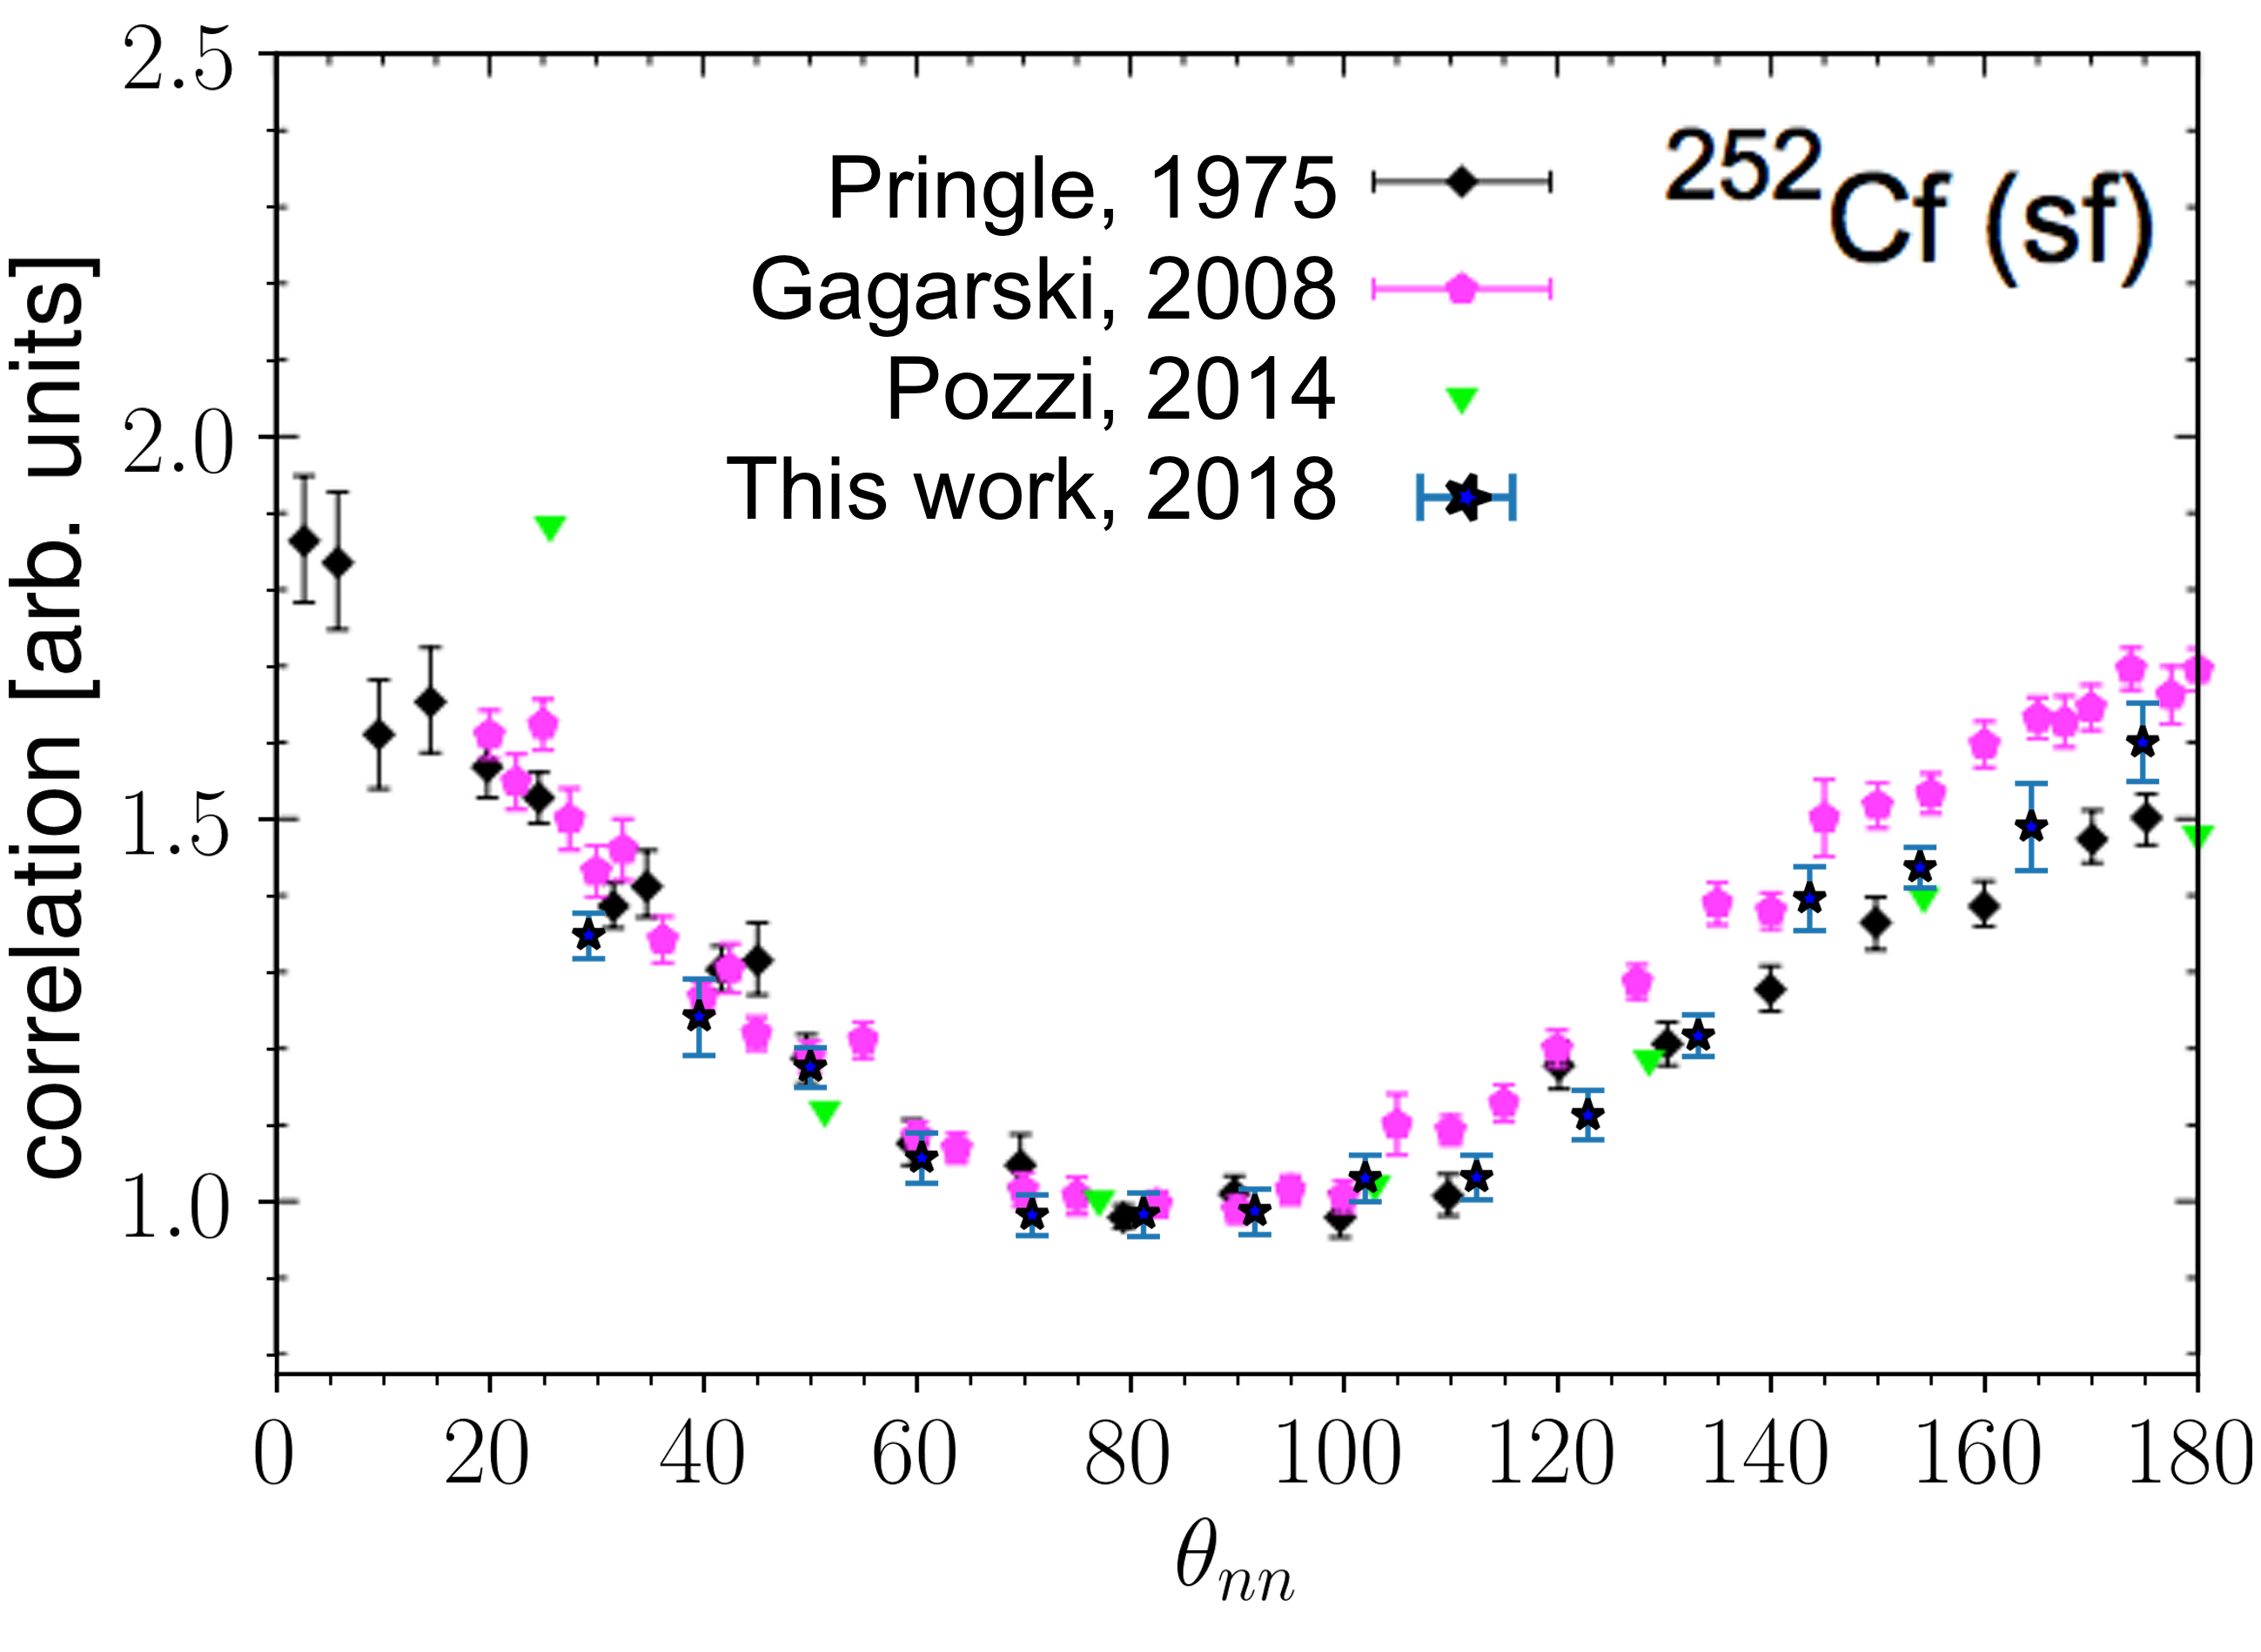
\includegraphics[width=0.45\textwidth]{Cf252_us_vs_them.png}
\caption{$\theta_{nn}$ distribution from the spontaneous fission of $^{252}$Cf.
 The neutron detection threshold for Pringle~\cite{1975Cf252}, Gagarski~\cite{2008CF252}, and Pozzi~\cite{Pozzi2016} is 0.425 MeV, 0.425 MeV, and 0.7 MeV, respectively, and for this work is 0.5 MeV.
}
\label{fig:Cf252_us_vs_them}
\end{figure}

\mysubsection{Considerations for Photofission}
\label{sec:level1}
The photofission reaction occurs during the de-excitation of a nucleus after the absorption of a photon.
For photon energies between 6 and 25 MeV, this absorption occurs primarily via the giant dipole resonance (GDR).
One distinct and useful aspect of photofission, relative to neutron-induced fission, is the low transfer of angular momentum to the nucleus, which gives rise to a simpler set of selection rules for the transfer of angular momentum.
For the photofission of even-even nuclei, excitation occurs primarily via electric dipole transitions, and to a lesser extent electric quadrupole transitions, which gives rise to anisotropies in the fission fragment angular distribution that are far more pronounced than for other types of fission~\cite{1977FragAss}.
These anisotropies are expressed in the angular distribution of emitted neutrons.
For these reasons, photofission is increasingly being used as a means to study sub-nuclear structures and the fundamentals of the fission process.
Such studies are needed in order to dial in various model parameters required for an accurate theoretical description of the fission process.